% Dissertation template designed by Scott P. Morton
% Middle Tennessee State University
% 5/1/2019

\documentclass[12pt, oneside]{memoir}

% Include these packages:
\usepackage{longtable}
\usepackage[utf8]{inputenc}
\usepackage{graphicx}
\usepackage[top=3.175cm, bottom=2.54cm, left=3.81cm, right=2.54cm]{geometry}	 % for margin requirements.
\usepackage{mathptmx}% http://ctan.org/pkg/mathptmx
\usepackage{setspace} % for double-spacing.
\usepackage{xifthen}%
\DoubleSpacing
\usepackage{lipsum}
\usepackage{tocloft}
\usepackage{color}
\usepackage{array}
\usepackage{stfloats}
\usepackage[export]{adjustbox}
\usepackage{multirow}
\usepackage{url}
\usepackage{changepage}
\usepackage{titlesec}
\usepackage{lscape}
\usepackage[table,xcdraw]{xcolor}
\usepackage{datetime}
\usepackage{natbib}
\usepackage{listings}
\usepackage{float}
\usepackage{amsmath}
\usepackage{textcomp}
\usepackage[colorlinks=true, linkcolor=black,citecolor=black,urlcolor=blue]{hyperref}
%\usepackage{color}

% Define the date format modifier
\newdateformat{mydate}{\monthname[\THEMONTH], \THEYEAR}

% - - Define code snippet configuration

% Make some specific colors for code snips
\definecolor{dkgreen}{rgb}{0,0.4,0}
\definecolor{ltgreen}{rgb}{0,0.6,0}
\definecolor{gray}{rgb}{0.5,0.5,0.5}
\definecolor{mygreen}{rgb}{0,0.6,0}
\definecolor{mygray}{rgb}{0.5,0.5,0.5}
\definecolor{mymauve}{rgb}{0.58,0,0.82}

% Force some setting specific to all programming languages, below there are specific language settings.
\lstset{ 
	backgroundcolor=\color{white},   % choose the background color; you must add \usepackage{color} or \usepackage{xcolor}; should come as last argument
	basicstyle=\footnotesize,        % the size of the fonts that are used for the code
	breakatwhitespace=false,         % sets if automatic breaks should only happen at whitespace
	breaklines=true,                 % sets automatic line breaking
	captionpos=b,                    % sets the caption-position to bottom
	commentstyle=\color{mygreen},    % comment style
	deletekeywords={...},            % if you want to delete keywords from the given language
	escapeinside={\%*}{*)},          % if you want to add LaTeX within your code
	extendedchars=true,              % lets you use non-ASCII characters; for 8-bits encodings only, does not work with UTF-8
	firstnumber=1000,                % start line enumeration with line 1000
	frame=single,	                   % adds a frame around the code
	keepspaces=true,                 % keeps spaces in text, useful for keeping indentation of code (possibly needs columns=flexible)
	keywordstyle=\color{blue},       % keyword style
	language=Python,                 % the language of the code
	% morekeywords={*,...},            % if you want to add more keywords to the set
	numbers=none,                    % where to put the line-numbers; possible values are (none, left, right)
	numbersep=5pt,                   % how far the line-numbers are from the code
	numberstyle=\tiny\color{mygray}, % the style that is used for the line-numbers
	rulecolor=\color{black},         % if not set, the frame-color may be changed on line-breaks within not-black text (e.g. comments (green here))
	showspaces=false,                % show spaces everywhere adding particular underscores; it overrides 'showstringspaces'
	showstringspaces=false,          % underline spaces within strings only
	showtabs=false,                  % show tabs within strings adding particular underscores
	stepnumber=2,                    % the step between two line-numbers. If it's 1, each line will be numbered
	stringstyle=\color{ltgreen},     % string literal style
	tabsize=2,	                   % sets default tabsize to 2 spaces
	title=\lstname                   % show the filename of files included with \lstinputlisting; also try caption instead of title
}


\lstdefinestyle{customc}{
	breaklines=true,
	frame=leftline,
	xleftmargin=\parindent,
	language=C,
	showstringspaces=false,
	%basicstyle=\footnotesize\ttfamily,
	keywordstyle=\bfseries\color{blue}, %{green!40!black},
	commentstyle=\itshape\color{purple!40!black},
	identifierstyle=\color{black},
	stringstyle=\color{ltgreen},
	tabsize=2
}

\lstdefinestyle{customcpp}{
	frame=tb,
	language=C++,
	aboveskip=3mm,
	belowskip=3mm,
	showstringspaces=false,
	columns=flexible,
	basicstyle={\small\ttfamily},
	numbers=none,
	numberstyle=\tiny\color{gray},
	keywordstyle=\color{blue},
	commentstyle=\color{dkgreen},
	stringstyle=\color{ltgreen},
	breaklines=true,
	breakatwhitespace=true,
	tabsize=3
}
% - - Define code snippet configuration

% - - Page Styling 
\counterwithout{figure}{chapter}
\counterwithout{table}{chapter}
\setlength\textfloatsep{18pt}

% - - Page numbering for mainmatter
\makeoddhead{plain}{}{}{\thepage}
\makeevenhead{plain}{}{}{\thepage}
\makeoddfoot{plain}{}{}{}
\makeevenfoot{plain}{}{}{}

% - - Page numbering for frontmatter
\makepagestyle{pter}
\makeoddhead{pter}{}{}{}
\makeevenhead{pter}{}{}{}
\makeoddfoot{pter}{}{\thepage}{}
\makeevenfoot{pter}{}{\thepage}{}
\pagestyle{pter}

% - - Styling for Section/Subsection/Subsubsection --
\titlespacing{\section}{0pt}{10pt}{-\parskip}
\titlespacing{\subsection}{0pt}{10pt}{-\parskip}
\titlespacing{\subsubsection}{0pt}{10pt}{-\parskip}
	% - - Section Headers
\titleformat{\section}{\normalfont\large\bfseries\filright}{}{0pt}{}
	% - - Subsection Headers
\titleformat{\subsection}{\normalfont\bfseries\itshape\filright}{}{0pt}{}
	% - - Subsection Headers
\titleformat{\subsubsection}{\normalfont\itshape\filright}{}{0pt}{}

% - - LOT LOF depth
\setcounter{lofdepth}{3}
\setcounter{lotdepth}{3}

% - - TOC
	%LOT LOF Bibliography styling
\AtBeginDocument{\addtocontents{toc}{\protect\thispagestyle{pter}}}
\AtBeginDocument{\addtocontents{lof}{\protect\thispagestyle{pter}}}
\AtBeginDocument{\addtocontents{lot}{\protect\thispagestyle{pter}}}
\renewcommand\bibname{\scshape\centerline{Bibliography}\global\def\bibname{\scshape Bibliography}}
%\setpnumwidth{4em}
 \renewcommand{\printtoctitle}{\centering\Large}
 \renewcommand*{\cftfigurename}{Figure \space}
 \renewcommand*{\cfttablename}{Table \space}
\renewcommand{\contentsname}{\scshape Table of Contents}
\renewcommand{\listfigurename}{\scshape List of Figures}
\renewcommand{\listtablename}{\scshape List of Tables}
	% - - TOC Chapter name styling
\renewcommand*{\cftchaptername}{\scshape Chapter\space}
\renewcommand*{\cftappendixname}{\scshape Appendix\space}
\renewcommand{\cftchapteraftersnum}{:}
\setlength{\cftchapternumwidth}{8mm}
\setsecnumdepth{chapter}

% Set figure and table numbering width in LOF, LOT
\setlength{\cftfigurenumwidth}{12mm}
\setlength{\cfttablenumwidth}{12mm}

% - - Chapter header styling
\makechapterstyle{Chapter}{
	\setlength{\beforechapskip}{-36.5pt}
	\setlength{\midchapskip}{5pt}
	\setlength{\afterchapskip}{10pt}
	\renewcommand{\afterchapternum}{ : }
	\renewcommand{\afterchaptertitle}{%
		\vskip 0.75\onelineskip \hrule\vskip\onelineskip}
	\renewcommand{\chaptitlefont}{\centering\normalfont\Large\scshape}
	\renewcommand{\chapnamefont}{\normalfont\Large\scshape}
	\renewcommand{\chapnumfont}{\normalfont\Large}
	\renewcommand{\thechapter}{\Roman{chapter}}
	\setcounter{tocdepth}{3}
}
\chapterstyle{Chapter}

% - - Appendix styling
\renewcommand*\cftappendixname{Appendix~}
\renewcommand{\appendixpagename}{\scshape \Large Appendices}
\renewcommand{\appendixtocname}{\scshape Appendices}

% - - Force table and figure number formats
\renewcommand{\thetable}{\arabic{chapter}.\arabic{table}}  
\renewcommand{\thefigure}{\arabic{chapter}.\arabic{figure}} 

% - - Force penalties for hanging/orphaned lines
\clubpenalty10000
\widowpenalty10000
\interlinepenalty=5000
\raggedbottom

% - - Force penalties for split references
\usepackage{etoolbox}
\patchcmd{\bibsetup}{\interlinepenalty=5000}{\interlinepenalty=10000}{}{}

\DoubleSpacing
\begin{document}

	\graphicspath{{./images/}}
	\bibliographystyle{apa}
	
	\frontmatter
	
	% - - - title page - - -
	\thispagestyle{empty}
	\begin{center}
	\vspace{2.54cm}\normalsize
	\begin{Large} \begin{SingleSpace}\bfseries \scshape A Dissertation / Thesis Template in \LaTeX \end{SingleSpace}\end{Large}
	%\vspace{2.54cm}\normalsize
	\vspace{1.27cm}\normalsize
	by\\Scott P. Morton
%	\vspace{2.54cm}\normalsize
	\vspace{1.27cm}\normalsize
	\begin{SingleSpace}
	A Dissertation (Thesis) Submitted in Partial Fulfillment of the Requirements for the Degree of\\
	\end{SingleSpace}
	\vspace{1.27cm}\normalsize
	%\begin{SingleSpace}
	The Degree\\in\\My Chosen Field\\
	%\end{SingleSpace}
	\vspace{1.27cm}\normalsize
	\vspace{1.27cm}\normalsize
	%\begin{SingleSpace}
	Middle Tennessee State University\\
	December, 2020
	%\mydate\today
	%\end{SingleSpace}
	%\vspace{2.54cm}\normalsize
	\vspace{1.27cm}\normalsize
	\begin{SingleSpace}
		%\hspace{11.0em}Dissertation Committee:
        Dissertation Committee:
	\end{SingleSpace}
	\begin{list}{}{\setlength{\leftmargin}{13.25em}\setlength{\itemsep}{0pt}}
		\item Dr. Greathearted, \emph{Chair}
		\item Dr. Yoda
		\item Dr. Dooalot
		\item Dr. Heliopolis
	\end{list}
	\end{center}
	\newpage
	% - - - Title Page - - -

	% - - - Dedications Page - - -
	\pagestyle{pter}
	\begin{vplace}[0.7]
		\begin{center}
		This page is optional. Students wishing to dedicate the thesis or dissertation to someone may do so using this page. This page does not include a heading, and the text should be brief and centered on the page. Pagination is centered, in lowercase Roman numerals.
		
		\end{center}
	\end{vplace}
	\newpage
	% - - - Dedications Page - - -

	% - - - Acknowedglements Page - - -
	\pagestyle{pter}
	\begin{center}
	\textbf{\Large\scshape Acknowledgments}
	\end{center}
	This page is optional and can be used to include brief statements of appreciation or recognition. This page has the heading “ACKNOWLEDGEMENTS,” and the heading must be centered and written in all capital letters. Pagination is centered, in lowercase Roman numerals.
	
	\newpage
	% - - - Acknowedglements Page - - -

	% - - - Abstract Page - - -
	\pagestyle{pter}
	\begin{center}
	\textbf{\Large\scshape Abstract}
	\end{center}
Every thesis or dissertation is required to include an abstract. This should be approximately 350 words for dissertations and 150 words for theses. The student and the committee will determine the content of the abstract. The page must be titled “ABSTRACT,” and the heading must be centered and written in all capital letters. Pagination is centered, in lowercase Roman numerals.

	
	\newpage
	% - - - Abstract Page - - -
	
	\tableofcontents*
	\clearpage
	
	\listoftables
    \clearpage

	\listoffigures
	\clearpage
	
	\mainmatter
	% - - - The Document - - -
	%    Copyright (C) 2020  Scott P. Morton (spm3c at mtmail.mtsu.edu)
%
%    This program is free software: you can redistribute it and/or modify
%    it under the terms of the GNU General Public License as published by
%    the Free Software Foundation, either version 3 of the License, or
%    (at your option) any later version.
%
%    This program is distributed in the hope that it will be useful,
%    but WITHOUT ANY WARRANTY; without even the implied warranty of
%    MERCHANTABILITY or FITNESS FOR A PARTICULAR PURPOSE.  See the
%    GNU General Public License for more details.
%
%    You should have received a copy of the GNU General Public License
%    along with this program.  If not, see <http://www.gnu.org/licenses/>.


% Dissertation template designed by Scott P. Morton
% Middle Tennessee State University
% 5/1/2019

\pagestyle{plain}
\chapter{Prologue} % single size step larger than text font
\renewcommand{\thetable}{\arabic{chapter}.\arabic{table}}  
\renewcommand{\thefigure}{\arabic{chapter}.\arabic{figure}} 

This is the introduction chapter, use it to introduce the audience to what this Thesis/Dissertation represents. Maybe your work is biology related and deals with proteins. Good graphics help assist with the introduction, see Figures \ref{fig:ala} and \ref{fig:ASN-ALA-CYS}. You might also want to mention your related publications.
%This research The sequence of amino acids that comprise a protein determines the shape and function, or more specifically, how the protein interacts with other proteins. Regardless of reference to the catalytic power of a protein, or the selectivity a certain protein has for interacting with another \citep{Garrett2010,Ma2011,AbdoolKarim2010}, the end result is a protein-protein interaction. 

\begin{figure}[h!]
\centering
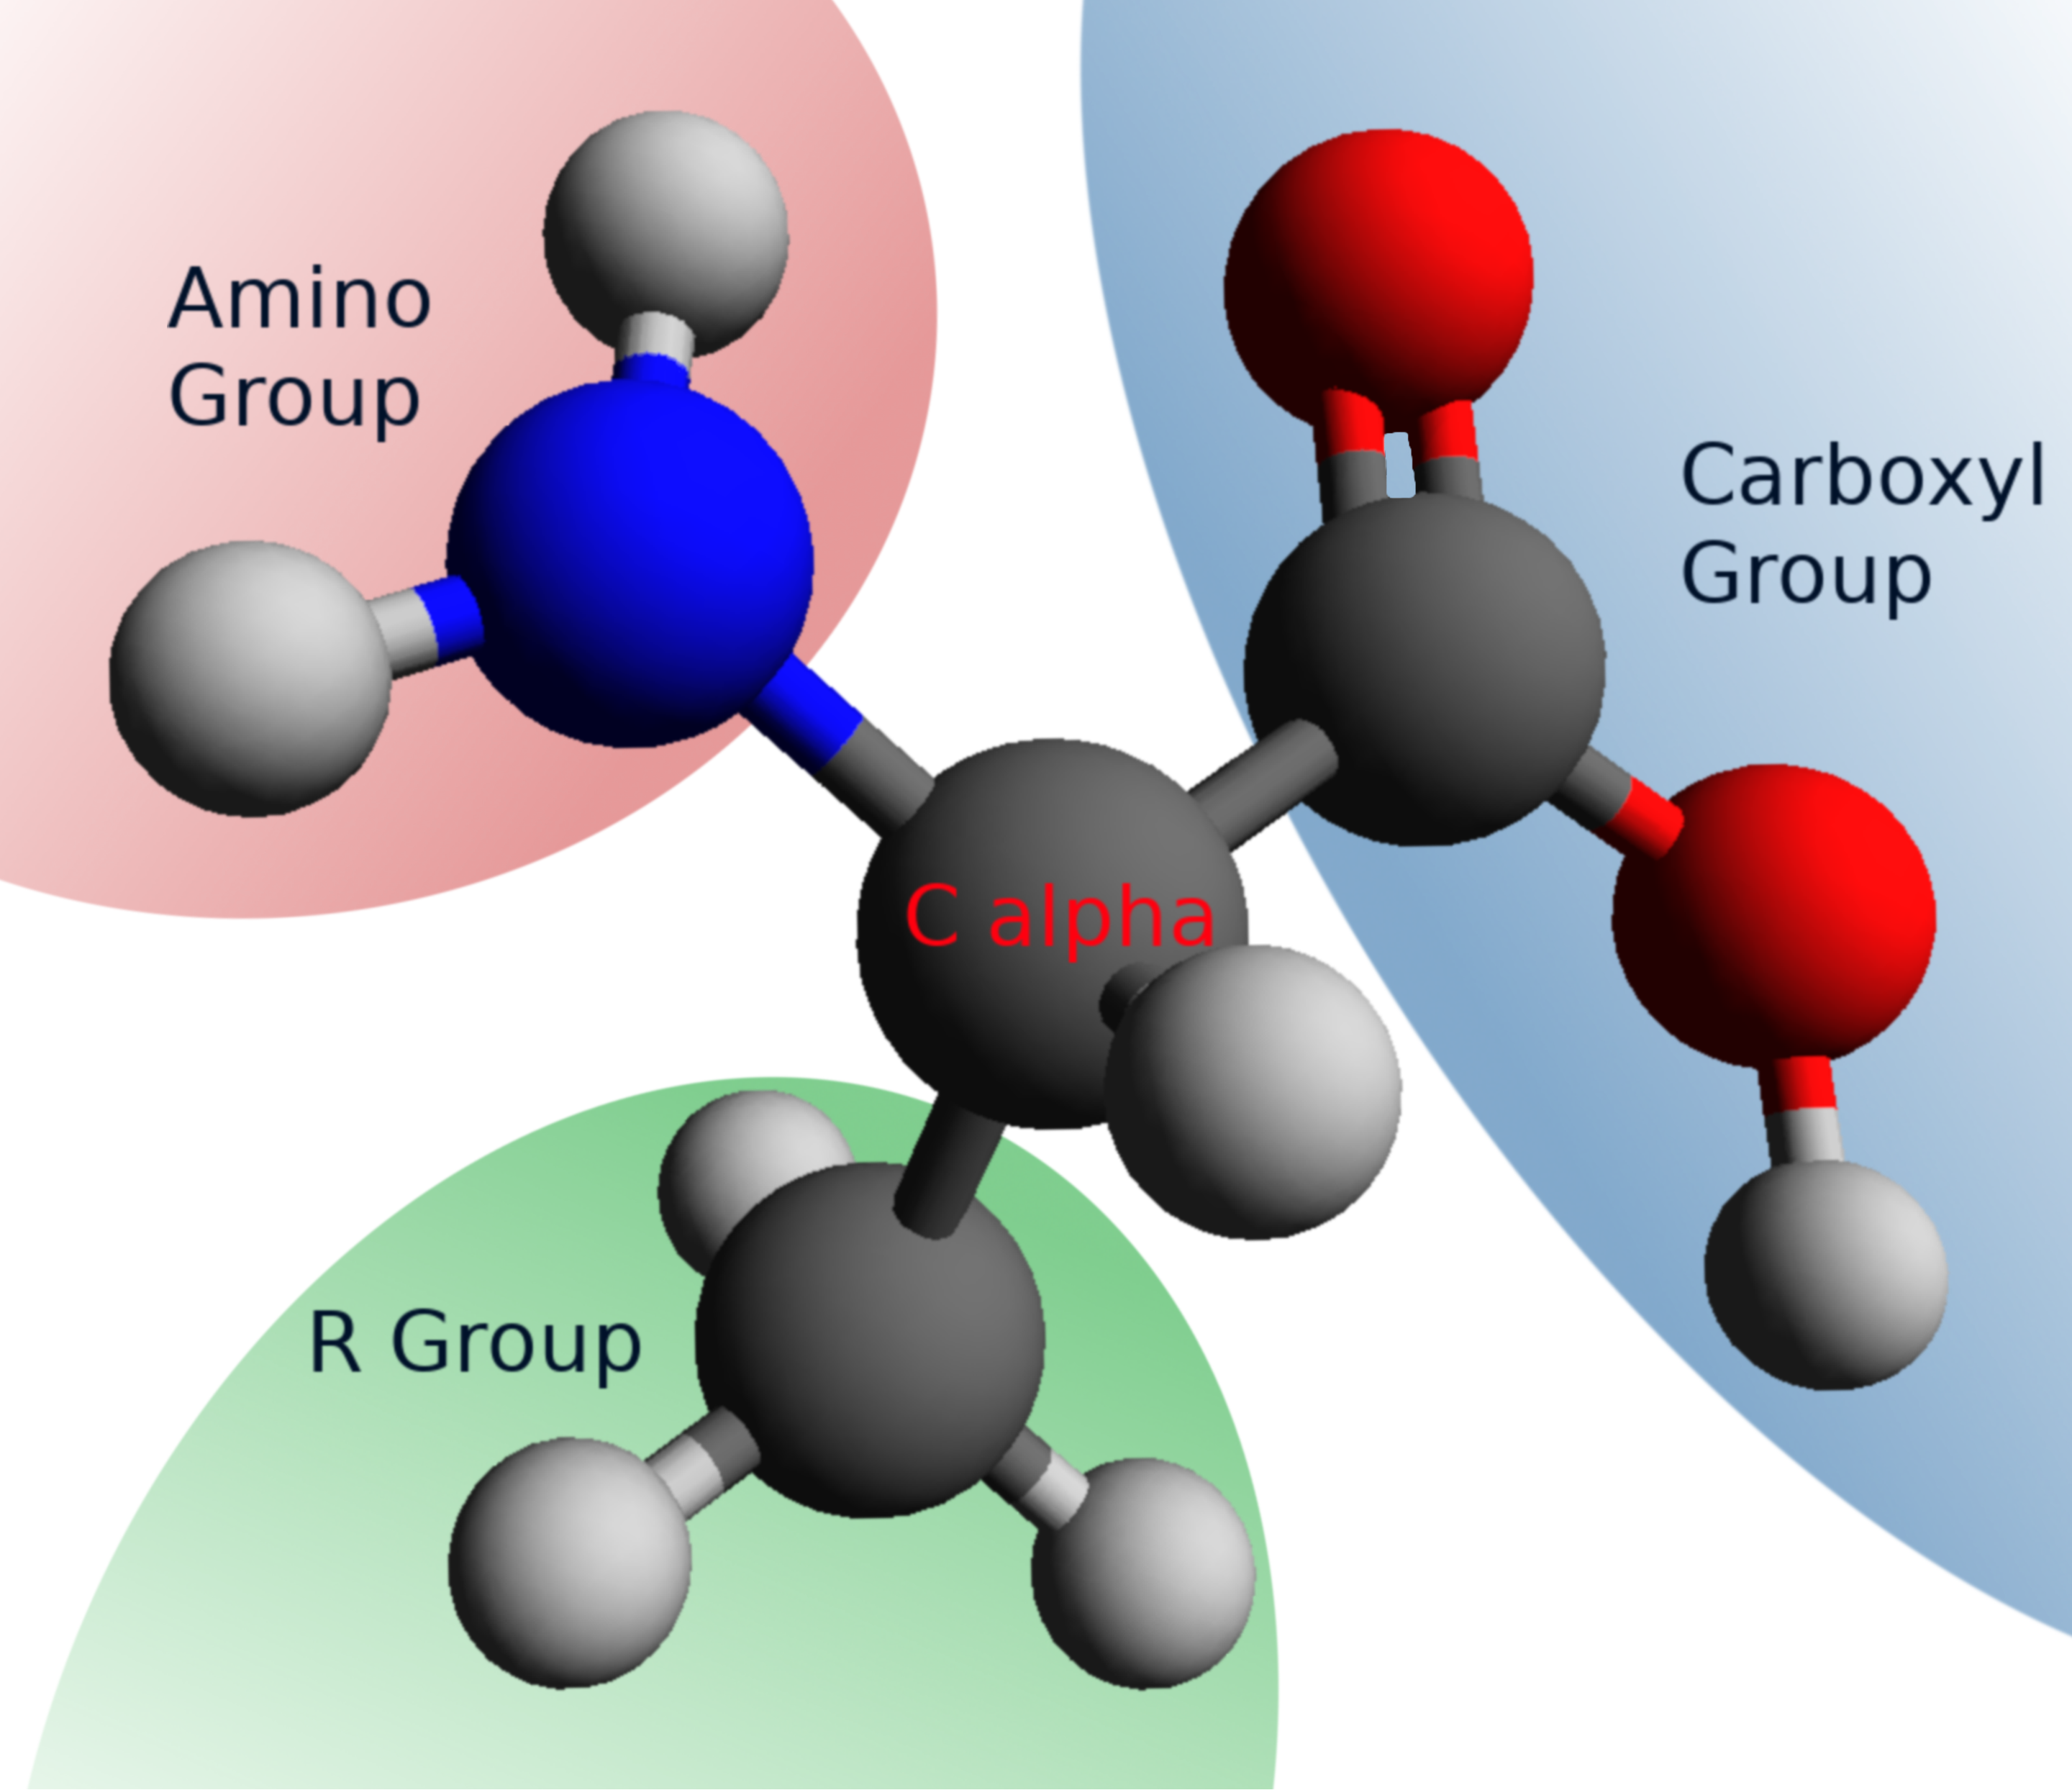
\includegraphics[width=0.7\linewidth]{images/ALA2}
\caption{The amino acid Alanine showing the amino group (red shading) bound to the alpha carbon $CH$ (center) that is bound to the carboxyl group (blue shading). The R group (green shading)  for Alanine is $CH_3$. Carbon is depicted as dark gray, hydrogen is light gray, oxygen is red and nitrogen is blue. Amino acid produced by Avogadro \citep{Hanwell2012}.}
\label{fig:ala}
\end{figure}

\begin{figure}[h!]
\centering
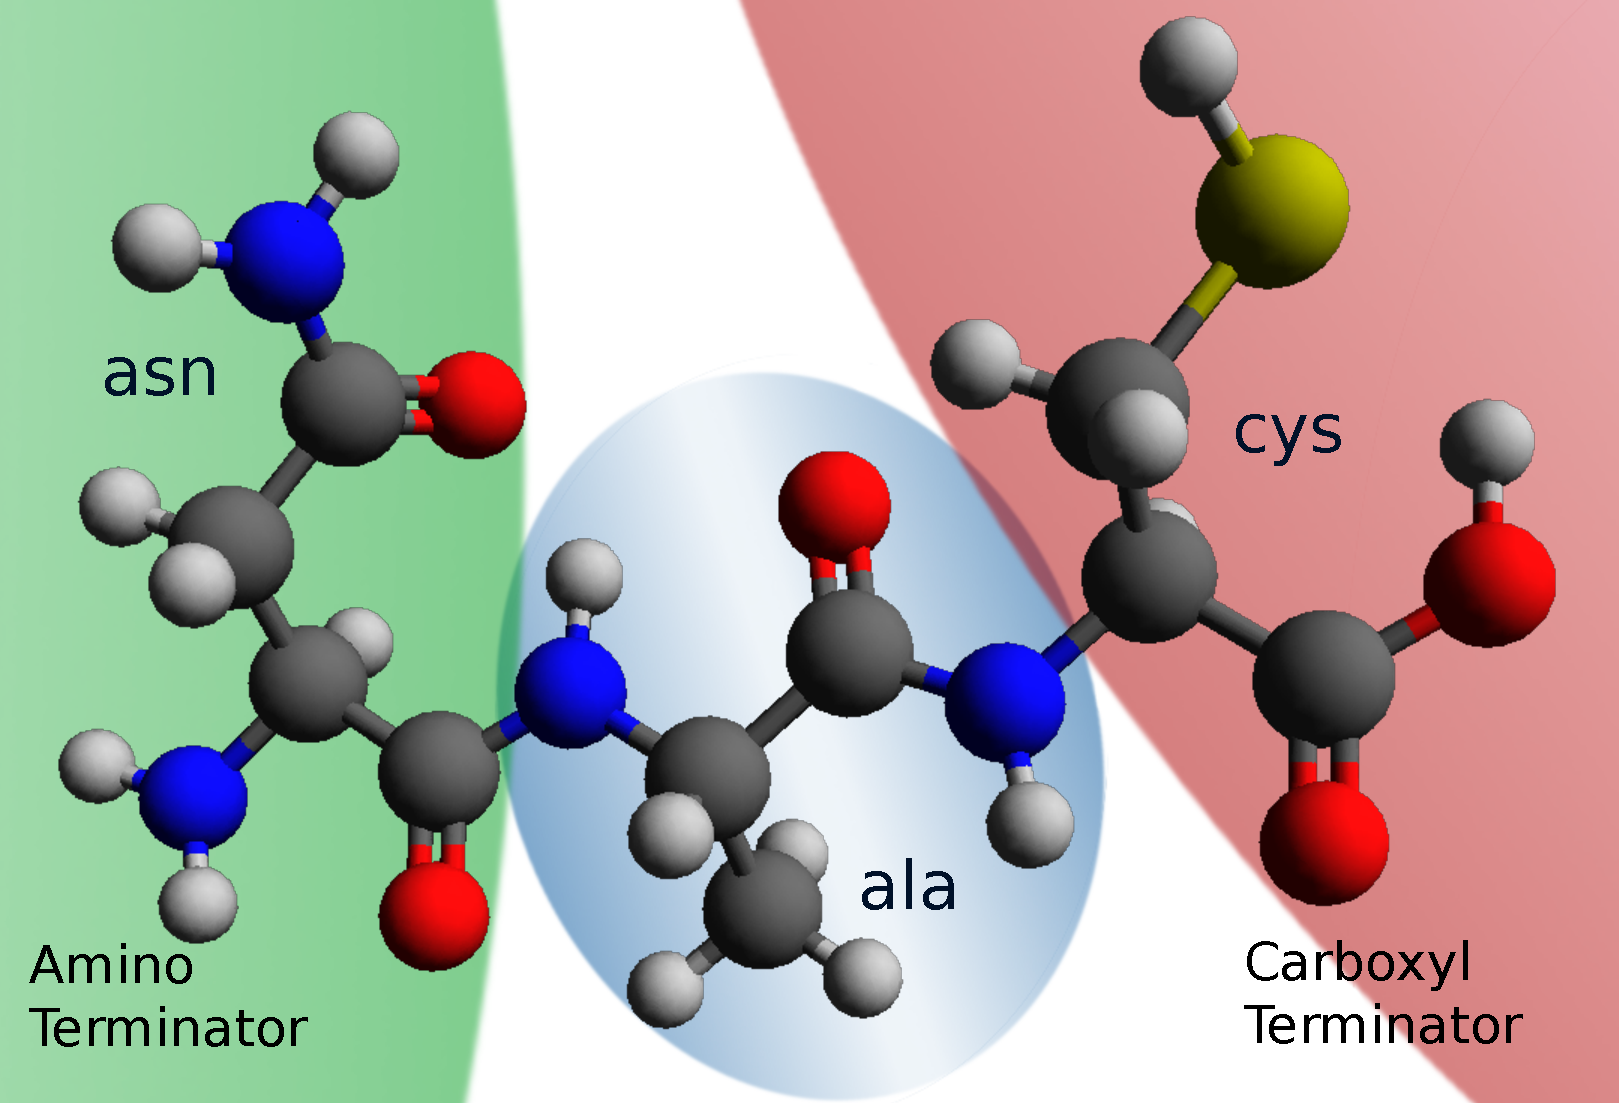
\includegraphics[width=0.7\linewidth]{images/ASN-ALA-CYS}
\caption{A simple protein chain with shading to distinguish each amino acid: Asparagine (green), Alanine (blue), and Cysteine (red). The amino terminal is to the left and the carboxyl terminal is to the right. Carbon is depicted as dark gray, hydrogen is light gray, oxygen is red, sulfur is yellow and nitrogen is blue. Protein chain produced by Avagadro \citep{Hanwell2012}.}
\label{fig:ASN-ALA-CYS}
\end{figure}


\noindent The following are related publications:

%\SingleSpacing
\begin{list}{}{}
	\item “Still Working on this Awesome Paper” (In preparation)

	\item Me, and You. “A Paper I Submitted and Currently Have a Preprint on BioRxiv.” BioRxiv, Cold Spring Harbor Laboratory, June 2020, the doc id and url. (Submitted for publication)

	\item Me, You, and Another ...

\end{list}
%\DoubleSpacing


	\clearpage
	\pagestyle{plain}
\chapter{Background Information} % single size step larger than text font
% for some specific formatting again just to be sure
\renewcommand{\thetable}{\arabic{chapter}.\arabic{table}}  
\renewcommand{\thefigure}{\arabic{chapter}.\arabic{figure}} 

\section{The First Subsection}
This is the background chapter, make the case for your dissertation. more graphics help and break it down by subject with subsections and subsubsections.
%\Spacing{3}

\section{Another Section}
More information on another aspect of the subject
	\clearpage
	\pagestyle{plain}
\chapter{Maybe a Chapter on How We Got the Data}
% again, reaffirm the formatting
\renewcommand{\thetable}{\arabic{chapter}.\arabic{table}}  
\renewcommand{\thefigure}{\arabic{chapter}.\arabic{figure}} 

This research extends upon previously developed methods to determine something about some thing. A figure here helps get the message across.

\section{My New Approach}
The pipeline of \citet{Stieh2013} is enhanced through the use of full structure assemblies, energy minimization, advanced compression techniques and a fully automatic execution environment. Notice the citation format, this is an inline citation used to call out a specific article, see the source code of this chapter. I may want to cite it as a matter of fact, in which case I want it to appear like this \citep{Stieh2013}. 

More graphics help get the message across

\subsection{Some Specific Details of Part A}
Structure modeling is facilitated through comparative modeling by Modeller \citep{Sali1993}. 

More Figures as needed
\subsection{Some Specific Details of Part B}
Once theoretical models are generated by Modeller, the structures are energy minimized by Gromacs \citep{Berendsen1995, Lindahl2001}.


	\clearpage
	\pagestyle{plain}
\chapter{Methods} 
% Reaffirm the formatting
\renewcommand{\thetable}{\arabic{chapter}.\arabic{table}}  
\renewcommand{\thefigure}{\arabic{chapter}.\arabic{figure}} 

\section{Background}
Some background information about your specific methods will help readers understand where all this started.
\subsection{Dynamic Electrophoretic Fingerprinting}
Electrophoretic mobility (EM) is an experimental measure of surface charge used to characterize and separate micro-organisms \citep{Mehrishi2002,Richmond1973}. Researchers hypothesized the method could be applied across saline and pH ranges relevant to mucosal environments where transmission is common and results in systemic infection. The method was employed to study trimeric gp120/gp41 from clade B HIV-1 strain BX08 \citep{Stieh2013} in the bound and unbound conformations by evaluating the difference between the two states. The results described surface charge variations across titrations indicating decreased gp120 surface charge in mucosal environments, complementing the positive charge of the CD4 receptor surface. This potentially could be the result of variations in gp120 protein structure and the interactions of surrounding solvent where blood plasma and mucous vary in pH and saline levels. This technique is used to validate the pipeline process in the methods that follow.


\section{My First New Method}
With a colorized table. I would suggest \href{https://www.tablesgenerator.com/}{https://www.tablesgenerator.com/} as a place to generate tables of this nature.
 
\begin{table}[]
	\caption{Visually impelling tables make a greater impact.}
	\label{tbl:BESISP}
	\centering
	\resizebox{14cm}{!}{%
		\begin{tabular}{|l|l|l|l|l|l|l|}
			\hline
			\multicolumn{7}{|c|}{\cellcolor[HTML]{CCCCCC}Unbound Data for Each Sequence}                                                                                                                                                                                                                                                         \\ \hline
			\multicolumn{1}{|l|}{\cellcolor[HTML]{DDDDDD}Model/pH}   & \multicolumn{1}{l|}{\cellcolor[HTML]{DDDDDD}3.0} & \multicolumn{1}{l|}{\cellcolor[HTML]{DDDDDD}3.1}  & \multicolumn{1}{l|}{\cellcolor[HTML]{DDDDDD}3.2} & \multicolumn{1}{l|}{\cellcolor[HTML]{DDDDDD}3.3}  & \multicolumn{1}{|l|}{\cellcolor[HTML]{DDDDDD}\dots}  & \multicolumn{1}{l|}{\cellcolor[HTML]{DDDDDD}9.0} \\ \hline
			\multicolumn{1}{|l|}{\cellcolor[HTML]{DDDDDD}Model\_1} & \multicolumn{1}{l|}{\cellcolor[HTML]{FFFC9E}0.008658}  & \multicolumn{1}{l|}{\cellcolor[HTML]{FFFC9E}-1.246752} & \multicolumn{1}{l|}{\cellcolor[HTML]{FFFC9E}0.441558}  & \multicolumn{1}{l|}{\cellcolor[HTML]{FFFC9E}1.229436}     & \multicolumn{1}{|l|}{\cellcolor[HTML]{FFFC9E}\dots}   & \multicolumn{1}{l|}{\cellcolor[HTML]{FFFC9E}-1.290042}   \\ \hline
			\multicolumn{1}{|l|}{\cellcolor[HTML]{DDDDDD}Model\_2}   & \multicolumn{1}{l|}{\cellcolor[HTML]{FFFC9E}0.017316}   & \multicolumn{1}{l|}{\cellcolor[HTML]{FFFC9E}1.25541}   & \multicolumn{1}{l|}{\cellcolor[HTML]{FFFC9E}-0.017316}  & \multicolumn{1}{l|}{\cellcolor[HTML]{FFFC9E}0.580086}     & \multicolumn{1}{|l|}{\cellcolor[HTML]{FFFC9E}\dots}    & \multicolumn{1}{l|}{\cellcolor[HTML]{FFFC9E}-1.16883}    \\ \hline
			\multicolumn{1}{|l|}{\cellcolor[HTML]{DDDDDD}\dots}  & \multicolumn{1}{l|}{\cellcolor[HTML]{FFFC9E}\dots}   & \multicolumn{1}{l|}{\cellcolor[HTML]{FFFC9E}\dots}  & \multicolumn{1}{l|}{\cellcolor[HTML]{FFFC9E}\dots}    & \multicolumn{1}{l|}{\cellcolor[HTML]{FFFC9E}\dots}    & \multicolumn{1}{|l|}{\cellcolor[HTML]{FFFC9E}\dots}   & \multicolumn{1}{l|}{\cellcolor[HTML]{FFFC9E}\dots}   \\ \hline
			\multicolumn{1}{|l|}{\cellcolor[HTML]{DDDDDD}Model\_N}  & \multicolumn{1}{l|}{\cellcolor[HTML]{FFFC9E}0.019243}   & \multicolumn{1}{l|}{\cellcolor[HTML]{FFFC9E}1.142856}   & \multicolumn{1}{l|}{\cellcolor[HTML]{FFFC9E}-1.55844}  & \multicolumn{1}{l|}{\cellcolor[HTML]{FFFC9E}1.549782}     & \multicolumn{1}{|l|}{\cellcolor[HTML]{FFFC9E}\dots}   & \multicolumn{1}{l|}{\cellcolor[HTML]{FFFC9E}1.090908}    \\ \hline
				\multicolumn{7}{|l|}{\cellcolor[HTML]{F3F3F3}} \\
				\multicolumn{7}{|l|}{\cellcolor[HTML]{F3F3F3}} \\
				 \hline
			\multicolumn{4}{|l|}{\cellcolor[HTML]{3166FF}}                                                                                                                                                                 & \multicolumn{3}{l|}{\cellcolor[HTML]{DDDDDD}}                                                                                                                                 \\ \cline{1-2}
			\cellcolor[HTML]{FFFC9E}Seq\_1 & \cellcolor[HTML]{FFFC9E}PCA & \multicolumn{1}{c|}{\cellcolor[HTML]{67FD9A}}                      & \multicolumn{1}{c|}{\cellcolor[HTML]{3166FF}}                                & \multicolumn{3}{l|}{\cellcolor[HTML]{DDDDDD}}                                                                                                                                 \\ \cline{1-2}
			\cellcolor[HTML]{FFFC9E}Seq\_2 & \cellcolor[HTML]{FFFC9E}PCA & \multicolumn{1}{c|}{\cellcolor[HTML]{67FD9A}}                      & \multicolumn{1}{c|}{\cellcolor[HTML]{3166FF}}                                & \multicolumn{3}{l|}{\cellcolor[HTML]{DDDDDD}}                                                                                                                                 \\ \cline{1-2}
			\cellcolor[HTML]{FFFC9E}\dots& \cellcolor[HTML]{FFFC9E}\dots & \multicolumn{1}{c|}{\cellcolor[HTML]{67FD9A}}                      & \multicolumn{1}{c|}{\cellcolor[HTML]{3166FF}}                                & \multicolumn{3}{l|}{\cellcolor[HTML]{DDDDDD}}                                                                                                                                 \\ \cline{1-2}
			\cellcolor[HTML]{FFFC9E}Seq\_N & \cellcolor[HTML]{FFFC9E}PCA & \multicolumn{1}{c|}{\multirow{-4}{*}{\cellcolor[HTML]{67FD9A}\begin{tabular}[c]{@{}l@{}}CSA\\of\\PC 1,2\end{tabular}}} & \multicolumn{1}{c|}{\multirow{-4}{*}{\cellcolor[HTML]{3166FF}\textbf{BESI}}} & \multicolumn{3}{l|}{\cellcolor[HTML]{DDDDDD}}                                                                                                                                 \\ \cline{1-2}
			\multicolumn{4}{|l|}{\cellcolor[HTML]{3166FF}}                                                                                                                                    & \multicolumn{3}{l|}{\multirow{-6}{*}{\cellcolor[HTML]{DDDDDD}\begin{tabular}[c]{@{}l@{}}BESI compares the first 2\\principal components of\\each sequence against the\\ first 2 principal components\\ of the control.\end{tabular}}} \\ 
			\hline
			
	\end{tabular}}
\end{table}

\subsection{Results}

These results are a product of \dots 


Check the source here to see how to manually insert hyphenation points in long character strings such as: Z242MPL25\-JAN03\-PCR23\-ENV\-1.1-DT and Z242MPL25\-JAN03\-PCR\-33ENV\-1.1-DNT gp120. It's a little painful at first and especially if you manuscript contains a lot of them. Some minor programming skills in Python \citep{Python1995} can make easy work of it.





\subsection{Discussion}

The results here have shown \dots


\section{My Next Method}
My next method and how data is extracted; visually represented in Figure \ref{fig:evm}.

\begin{figure}
\centering
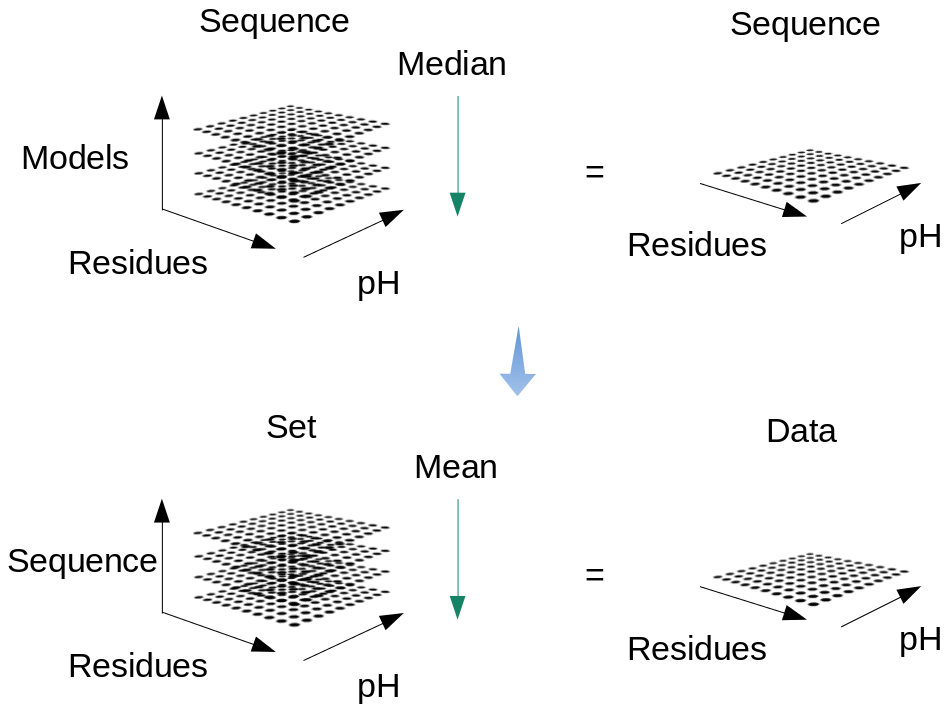
\includegraphics[width=0.7\linewidth]{images/EVM}
\caption{Visualization of the process to extract variance data from residue electrostatics. Models of residue data are reduced to 2 dimensions by taking the median of the set across models/residue to eliminate the effects of outliers on the data. Once each seqence/model set is processed, the mean across the sequence set is taken to produce the residue data for which the variance is extracted for each residue across the pH range.}
\label{fig:evm}
\end{figure}


\subsection{Results}
The first set of results comes from \dots

For the purposes of expressing these data, all theoretical data will be normalized for clarity using:
\[ x' = \dfrac {x - set_{min}}{set_{max} - set_{min}}
 \]
Where $x$ is the theoretical value, $set_{min}$ is the minimum value of all theoretical data produced, $set_{max}$ is the maximum value of all theoretical data produced, and $x'$ is the normalized value returned.

\subsection{Discussion}
Motifs provide no evidence that the range of \dots

\section{Comparing Soandso to Supervised Machine Learning}
This section is presented as validation of the unsupervised methods \dots 

\subsubsection{Binary Classifier}
Figure \ref{fig:binaryclassifier} shows the model construct for the binary classifier using sixty-one inputs with a one hundred and twenty eight node hidden layer to a single node output. Figure \ref{fig:binary-ann} provides a visual representation of the binary classifier. Dropout layers are only used during training to prevent over-fitting the data and are not depicted in the figure. The neural network is dense (fully meshed) and utilizes Rectified Linear Unit (ReLU) activation for the input and hidden layers. Output is sigmoid activated to complete the binary classifier.
\begin{figure}[h!]
	\lstset{style=customc, language=Python}
	\begin{lstlisting}
model = keras.Sequential(
    [
    layers.Dense(128, input_dim=61, activation='relu'),
    layers.Dropout(0.5),
    layers.Dense(128, activation='relu'),
    layers.Dropout(0.5),
    layers.Dense(1, activation='sigmoid')
    ]
    )

model.compile(loss='binary_crossentropy',
              optimizer='rmsprop',
              metrics=['accuracy'])

history = model.fit(x_train, y_train, 
                    epochs=100, batch_size=50,
                    validation_data=(x_val, y_val),
                    verbose=1)

test_data = np.genfromtxt('inputdata.txt', delimiter=' ')
test_data_labels = np.genfromtxt('sequence.list', delimiter=' ')

results = model.predict(test_data)
	\end{lstlisting}
	\caption{Model construct of a binary classifier using 61 inputs tied to a 128 node hidden layer that feeds a single output node.}\
	\label{fig:binaryclassifier}
\end{figure}

\begin{figure}
\centering
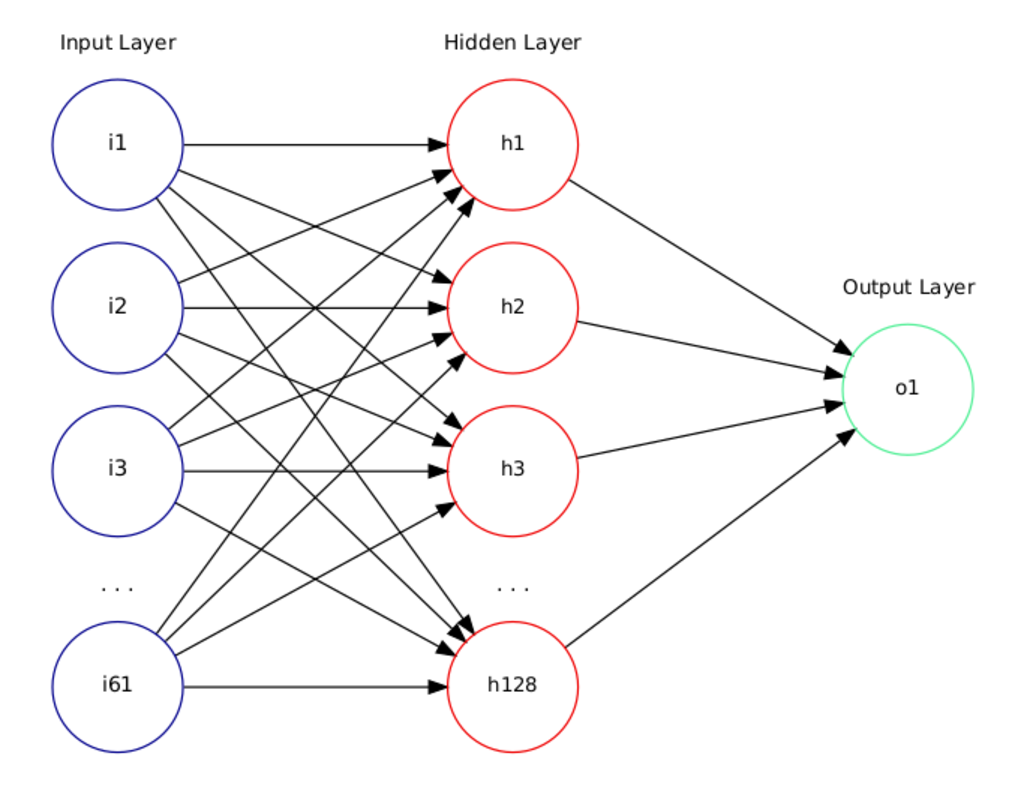
\includegraphics[width=0.7\linewidth]{images/binary-ann}
\caption{Graphic representation of binary classifier showing individual layers. Dropout layers are not expressed and are only used during training to control over and under fitting.}
\label{fig:binary-ann}
\end{figure}

\subsection{Results}
Scoring by the binary classifier can be see in Table \ref{tab:binariescores} for all 252 \dots

This is an example of a multi-page table:

{\footnotesize \centering
\begin{longtable}{|l|c|l|c|}
\kill

\caption{Scoring from binary classifier showing under-fitting by the neural network.  \label{tab:binariescores}} \\
\hline
\textbf{Sequence} & \textbf{Score} & \textbf{Sequence} & \textbf{Score} \\ \hline
\endfirsthead
\multicolumn{4}{c}%
{\tablename\ \thetable\ -- \textit{Continued from previous page}} \\ \hline
\textbf{Sequence} & \textbf{Score} & \textbf{Sequence} & \textbf{Score} \\ \hline
\endhead
\multicolumn{4}{r}%
{\tablename\ \thetable\ -- \textit{Continued on next page}} \\ \hline
\endfoot
\hline
\endlastfoot
                            Z238FSW15A6\_plasmid\_6v 	&	0.9819	&	                               Z201FPL07feb03102-1 	&	1	\\ \hline
                            Z238FSW15G4\_plasmid\_4i 	&	0.9999	&	                               Z201FPL07feb03103-1 	&	1	\\ \hline
                           Z238FSW15H8\_plasmid\_3ii 	&	1	&	                               Z201FPL07feb03105-1 	&	1	\\ \hline
                               Z238FSW29oct0215A11 	&	1	&	                                Z201FPL07feb0350-2 	&	1	\\ \hline
                               Z238FSW29oct0215A6v 	&	0.9767	&	                                Z201FPL07feb0351-1 	&	0.8955	\\ \hline
                                Z238FSW29oct0215G4 	&	0.9999	&	                                Z201FPL07feb0368-2 	&	1	\\ \hline
                                Z238FSW29oct0215H8 	&	1	&	                                Z201FPL07feb0372-1 	&	1	\\ \hline
                               Z238MPL17\_plasmid\_a 	&	0.8942	&	                                Z201FPL07feb0390-1 	&	1	\\ \hline
                                Z238MPL9\_plasmid\_c 	&	0.3827	&	                            Z201FPL100\_plasmid\_8-1 	&	1	\\ \hline
                         Z242FPL25JAN03PCR23ENV1.1 	&	0.9998	&	                            Z201FPL102\_plasmid\_7-1 	&	1	\\ \hline
                          Z242FPL25JAN03PCR8ENV1.1 	&	1	&	                            Z201FPL103\_plasmid\_4-1 	&	1	\\ \hline
                           Z242FPL25jan038\_plasmid 	&	1	&	                            Z201FPL105\_plasmid\_3-1 	&	1	\\ \hline
                                  Z242MPL25JAN0326 	&	0.8888	&	                             Z201FPL50\_plasmid\_5-2 	&	1	\\ \hline
                                Z242MPL25JAN0327-1 	&	1	&	                             Z201FPL51\_plasmid\_1-1 	&	0.913	\\ \hline
                                Z242MPL25JAN0327-2 	&	0.9999	&	                             Z201FPL68\_plasmid\_6-2 	&	1	\\ \hline
                                Z242MPL25JAN0327-3 	&	1	&	                             Z201FPL72\_plasmid\_9-1 	&	1	\\ \hline
                      Z242MPL25JAN03PCR23ENV1.1-DT 	&	1	&	                               Z201FPL7FEB03ENV1.8 	&	1	\\ \hline
                     Z242MPL25JAN03PCR33ENV1.1-DNT 	&	0.0016	&	                               Z201FPL7FEB03ENV2.1 	&	1	\\ \hline
                          Z242MPL25jan0323\_plasmid 	&	1	&	                               Z201FPL7FEB03ENV3.3 	&	1	\\ \hline
                          Z242MPL25jan0326\_plasmid 	&	0.9648	&	                               Z201FPL7FEB03ENV4.1 	&	1	\\ \hline
                      Z242MPL25jan0328\_plasmid\_8-1 	&	1	&	                               Z201FPL7FEB03ENV5.2 	&	1	\\ \hline
                      Z242MPL25jan0328\_plasmid\_8-2 	&	1	&	                               Z201FPL7FEB03ENV6.1 	&	1	\\ \hline
                      Z242MPL25jan0328\_plasmid\_8-3 	&	0.9998	&	                               Z201FPL7FEB03ENV7.1 	&	0.8914	\\ \hline
                          Z242MPL25jan0333\_plasmid 	&	0.0018	&	                             Z201FPL90\_plasmid\_2-1 	&	1	\\ \hline
                                 Z242MPL26\_plasmid 	&	0.9942	&	                             Z201FSW07feb03DNA13D1 	&	1	\\ \hline
                             Z242MPL28\_plasmid\_8-1 	&	1	&	                         Z201FSWDNA13D1\_plasmid\_4i 	&	1	\\ \hline
                             Z242MPL28\_plasmid\_8-2 	&	1	&	                               Z201MPB7FEB03ENV2.1 	&	1	\\ \hline
                             Z242MPL28\_plasmid\_8-3 	&	1	&	                               Z201MPB7FEB03ENV4.1 	&	1	\\ \hline
                           Z292FCA12A52\_plasmid\_9v 	&	1	&	                               Z201MPB7FEB03ENV5.1 	&	0.9999	\\ \hline
                               Z292FCA24may0512A52 	&	1	&	                                 Z201MPL07feb0352a 	&	1	\\ \hline
                    Z292FCA24may0512A52\_plasmid\_9v 	&	1	&	                                Z201MPL07feb0352aa 	&	0.9995	\\ \hline
                    Z292FCA24may0512A58\_plasmid\_6v 	&	0.9656	&	                                 Z201MPL07feb0352e 	&	0.9998	\\ \hline
                  Z292FCA24may0512D10\_plasmid\_5iii 	&	1	&	                                 Z201MPL07feb0384c 	&	0.9999	\\ \hline
                         Z292FCF12E26\_plasmid\_10iv 	&	1	&	                               Z201MPL52\_plasmid\_a 	&	0.9999	\\ \hline
                    Z292FCF24may0512D18\_plasmid\_4i 	&	1	&	                              Z201MPL52\_plasmid\_aa 	&	0.9999	\\ \hline
                               Z292FCF24may0512E26 	&	1	&	                               Z201MPL52\_plasmid\_e 	&	0.9998	\\ \hline
                  Z292FCF24may0512E26\_plasmid\_10iv 	&	1	&	                               Z201MPL7FEB03ENV2.1 	&	0.9998	\\ \hline
                     Z292FPL24may05105\_plasmid\_5-1 	&	1	&	                               Z201MPL7FEB03ENV3.1 	&	1	\\ \hline
                     Z292FPL24may05136\_plasmid\_7-1 	&	1	&	                               Z201MPL7FEB03ENV4.1 	&	1	\\ \hline
                     Z292FPL24may05152\_plasmid\_1-3 	&	0.9999	&	                               Z201MPL84\_plasmid\_c 	&	0.9957	\\ \hline
                     Z292FPL24may05160\_plasmid\_4-1 	&	1	&	                              Z205FPB27MAR03ENV1.1 	&	0.8165	\\ \hline
                     Z292FPL24may05164\_plasmid\_9-2 	&	1	&	                              Z205FPB27MAR03ENV4.2 	&	0.7305	\\ \hline
                     Z292FPL24may05172\_plasmid\_6-1 	&	1	&	                              Z205FPL27MAR03ENV4.1 	&	0.019	\\ \hline
                      Z292FPL24may0535\_plasmid\_3-3 	&	1	&	                              Z205FPL27MAR03ENV5.2 	&	1	\\ \hline
                    Z292FSW24may0512E12\_plasmid\_3v 	&	0.9996	&	                              Z205FPL27MAR03ENV6.3 	&	0.6004	\\ \hline
                    Z292FSW24may0512E20\_plasmid\_2i 	&	1	&	                              Z205MPB27MAR03ENV4.1 	&	1	\\ \hline
                              Z292MPL113\_plasmid\_e 	&	1	&	                              Z205MPB27MAR03ENV6.1 	&	1	\\ \hline
                              Z292MPL150\_plasmid\_b 	&	1	&	                              Z205MPB27MAR03ENV9.1 	&	0.0816	\\ \hline
                       Z292MPL24may05113\_plasmid\_e 	&	1	&	                            Z205MPL27MAR03ENV1.1NF 	&	1	\\ \hline
                                Z292MPL24may05113e 	&	1	&	                              Z205MPL27MAR03ENV2.3 	&	0.341	\\ \hline
                       Z292MPL24may05150\_plasmid\_b 	&	1	&	                            Z205MPL27MAR03ENV3.1NF 	&	0.9999	\\ \hline
                                Z292MPL24may05150b 	&	1	&	                              Z205MPL27MAR03ENV6.3 	&	1	\\ \hline
                         R56FPL21apr05B6\_plasmid\_a 	&	0.9777	&	                               Z216FC17jan04RNAB37 	&	0.9996	\\ \hline
                         R56FPL21apr05B6\_plasmid\_b 	&	0.9807	&	                              Z216FCF17jan04RNAB44 	&	0.0097	\\ \hline
                         R56FPL21apr05E7\_plasmid\_a 	&	0.5807	&	                       Z216FCFRNA11B44\_plasmid\_2iv 	&	0.0064	\\ \hline
                         R56FPL21apr05E7\_plasmid\_b 	&	0.9906	&	                         Z216FCRNA11B37\_plasmid\_7i 	&	0.9998	\\ \hline
                      R56MCA21aug0516\_plasmid\_9iii 	&	0.9999	&	                              Z216FPB112\_plasmid\_e 	&	1	\\ \hline
                         R56MCA21aug053\_plasmid\_5i 	&	1	&	                               Z216FPB85\_plasmid\_f 	&	0.9289	\\ \hline
                       R56MCA21aug056\_plasmid\_6iii 	&	1	&	                               Z216FPB98\_plasmid\_e 	&	0.9447	\\ \hline
                        R56MCF21aug0511\_plasmid\_1v 	&	1	&	                            Z216FPL129\_plasmid\_6-1 	&	1	\\ \hline
                       R56MCF21aug0514\_plasmid\_2iv 	&	1	&	                            Z216FPL138\_plasmid\_8-3 	&	0.9963	\\ \hline
                       R56MCF21aug0519\_plasmid\_3ii 	&	1	&	                                Z216FPL17jan04112e 	&	1	\\ \hline
                       R56MPL21apr05C2\_plasmid\_7-1 	&	1	&	                                 Z216FPL17jan04129 	&	1	\\ \hline
                       R56MPL21apr05C5\_plasmid\_6-4 	&	1	&	                                 Z216FPL17jan04138 	&	0.9872	\\ \hline
                       R56MPL21apr05G5\_plasmid\_5-3 	&	1	&	                                 Z216FPL17jan04190 	&	0.9994	\\ \hline
                       R56MPL21apr05H3\_plasmid\_1-3 	&	1	&	                                   Z216FPL17jan046 	&	0.0008	\\ \hline
                       R56MPL21apr05K4\_plasmid\_4-1 	&	1	&	                                  Z216FPL17jan0483 	&	0.0069	\\ \hline
                       R56MPL21apr05K6\_plasmid\_2-4 	&	1	&	                                 Z216FPL17jan0485f 	&	0.9793	\\ \hline
                       R56MPL21apr05P5\_plasmid\_8-1 	&	1	&	                                  Z216FPL17jan0492 	&	1	\\ \hline
                              Z153FPB13MAR02ENV1.1 	&	0.828	&	                                 Z216FPL17jan0498e 	&	0.8215	\\ \hline
                              Z153FPB13MAR02ENV2.1 	&	0.9979	&	                            Z216FPL190\_plasmid\_5-1 	&	0.9999	\\ \hline
                              Z153FPB13MAR02ENV3.1 	&	0.3384	&	                              Z216FPL6\_plasmid\_4-4 	&	0.0028	\\ \hline
                              Z153FPB13MAR02ENV4.1 	&	0.9996	&	                             Z216FPL83\_plasmid\_7-2 	&	0.1336	\\ \hline
                              Z153FPB13MAR02ENV5.1 	&	0.9989	&	                             Z216FPL92\_plasmid\_1-1 	&	0.9999	\\ \hline
                              Z153FPL13MAR02ENV1.1 	&	0.9033	&	                               Z216FSW17jan04DNA15 	&	0.975	\\ \hline
                              Z153FPL13MAR02ENV2.1 	&	0.2734	&	                         Z216FSWDNA11I5\_plasmid\_5v 	&	0.9916	\\ \hline
                              Z153FPL13MAR02ENV3.1 	&	0.0002	&	                                Z216MPL133\_plasmid 	&	0.9964	\\ \hline
                              Z153FPL13MAR02ENV4.1 	&	0.9996	&	                              Z221FPB7MAR03ENV10.3 	&	1	\\ \hline
                              Z153FPL13MAR02ENV5.1 	&	0.0015	&	                              Z221FPB7MAR03ENV11.3 	&	1	\\ \hline
                              Z153FPL13MAR02ENV6.1 	&	0.0014	&	                               Z221FPB7MAR03ENV6.4 	&	1	\\ \hline
                              Z153MPB13MAR02ENV1.1 	&	0.9998	&	                               Z221FPB7MAR03ENV9.1 	&	0.935	\\ \hline
                              Z153MPB13MAR02ENV2.1 	&	0.8576	&	                                  Z221FPL08mar0335 	&	0.9796	\\ \hline
                              Z153MPB13MAR02ENV3.1 	&	0.9998	&	                                  Z221FPL08mar0344 	&	0.0004	\\ \hline
                              Z153MPB13MAR02ENV4.1 	&	1	&	                                  Z221FPL08mar0348 	&	0.4223	\\ \hline
                              Z153MPB13MAR02ENV5.1 	&	0.9999	&	                                  Z221FPL08mar0351 	&	0.9989	\\ \hline
                              Z153MPL13MAR02ENV1.1 	&	0.9996	&	                                  Z221FPL08mar0355 	&	0.0619	\\ \hline
                              Z153MPL13MAR02ENV2.1 	&	0.9995	&	                                  Z221FPL08mar0371 	&	0.9597	\\ \hline
                              Z153MPL13MAR02ENV3.1 	&	0.9631	&	                                  Z221FPL08mar0380 	&	1	\\ \hline
                              Z153MPL13MAR02ENV4.1 	&	0.9997	&	                             Z221FPL35\_plasmid\_7-1 	&	0.8827	\\ \hline
                              Z153MPL13MAR02ENV5.1 	&	0.9996	&	                             Z221FPL44\_plasmid\_4-1 	&	0.0008	\\ \hline
                              Z185FPB24AUG02ENV1.1 	&	0	&	                             Z221FPL48\_plasmid\_5-1 	&	0.3918	\\ \hline
                              Z185FPB24AUG02ENV2.1 	&	0	&	                             Z221FPL51\_plasmid\_2-2 	&	0.9996	\\ \hline
                              Z185FPB24AUG02ENV3.1 	&	0	&	                             Z221FPL55\_plasmid\_6-2 	&	0.0259	\\ \hline
                              Z185FPB24AUG02ENV4.1 	&	0	&	                             Z221FPL71\_plasmid\_9-1 	&	0.9746	\\ \hline
                              Z185FPB24AUG02ENV5.1 	&	0	&	                               Z221FPL7MAR03ENV1.2 	&	0.9677	\\ \hline
                              Z185FPL17AUG02ENV1.1 	&	0.0003	&	                              Z221FPL7MAR03ENV10.4 	&	0.9999	\\ \hline
                              Z185FPL17AUG02ENV2.1 	&	0	&	                               Z221FPL7MAR03ENV2.3 	&	1	\\ \hline
                              Z185FPL17AUG02ENV3.1 	&	0.0018	&	                               Z221FPL7MAR03ENV3.3 	&	0.9987	\\ \hline
                              Z185FPL17AUG02ENV4.1 	&	0	&	                             Z221FPL80\_plasmid\_8-3 	&	1	\\ \hline
                              Z185FPL17AUG02ENV5.1 	&	0	&	                            Z221FSW08mar0314H16iii 	&	0.7743	\\ \hline
                              Z185MPB17AUG02ENV1.2 	&	0.0038	&	                             Z221FSW08mar0314H16iv 	&	0.9668	\\ \hline
                              Z185MPB17AUG02ENV1.5 	&	0.0021	&	                         Z221FSW14H16\_plasmid\_6iii 	&	0.9665	\\ \hline
                              Z185MPB17AUG02ENV7.4 	&	0	&	                        Z221FSW14H16iv\_plasmid\_6iv 	&	0.9941	\\ \hline
                              Z185MPB17AUG02ENV7.5 	&	0	&	                               Z221MPB7MAR03ENV4.1 	&	0.9832	\\ \hline
                              Z185MPB17AUG02ENV7.6 	&	0	&	                               Z221MPB7MAR03ENV5.4 	&	0.8951	\\ \hline
                              Z185MPB17AUG02ENVB17 	&	0	&	                               Z221MPB7MAR03ENV6.4 	&	0.2915	\\ \hline
                               Z185MPB17AUG02ENVB6 	&	0	&	                                 Z221MPL08mar0375a 	&	0.8709	\\ \hline
                              Z185MPB17AUG02ENVC17 	&	0	&	                                 Z221MPL08mar0375f 	&	0.9939	\\ \hline
                              Z185MPB17AUG02ENVC18 	&	0	&	                               Z221MPL75\_plasmid\_a 	&	0.9284	\\ \hline
                               Z185MPB17AUG02ENVC8 	&	0.0034	&	                               Z221MPL75\_plasmid\_f 	&	0.9941	\\ \hline
                                Z201FCA07feb0313C8 	&	0.9999	&	                               Z221MPL7MAR03ENV2.1 	&	0.9861	\\ \hline
                            Z201FCA07feb03DNA13G10 	&	1	&	                               Z221MPL7MAR03ENV4.2 	&	0.9195	\\ \hline
                          Z201FCA13C8\_plasmid\_2iii 	&	0.9999	&	                               Z221MPL7MAR03ENV6.4 	&	0.8982	\\ \hline
                        Z201FCADNA13G10\_plasmid\_6i 	&	1	&	                            Z238FCA15C6\_plasmid\_1v 	&	0.8263	\\ \hline
                            Z201FCF07feb03DNA13C18 	&	1	&	                                Z238FCA29oct0215C6 	&	0.8369	\\ \hline
                            Z201FCF07feb03DNA13G13 	&	1	&	                          Z238FCF15A39\_plasmid\_9ii 	&	1	\\ \hline
                            Z201FCF07feb03DNA13H13 	&	0.9999	&	                          Z238FCF15C13\_plasmid\_2ii 	&	1	\\ \hline
                             Z201FCF07feb03DNA13H9 	&	0.4086	&	                               Z238FCF29oct0215A39 	&	1	\\ \hline
                       Z201FCFDNA13C18\_plasmid\_3ii 	&	1	&	                               Z238FCF29oct0215C13 	&	1	\\ \hline
                        Z201FCFDNA13G13\_plasmid\_7i 	&	1	&	                             Z238FPL12\_plasmid\_1-2 	&	1	\\ \hline
                       Z201FCFDNA13H13\_plasmid\_10i 	&	0.9991	&	                             Z238FPL16\_plasmid\_2-3 	&	1	\\ \hline
                         Z201FCFDNA13H9\_plasmid\_8v 	&	0.3429	&	                                  Z238FPL29nov0212 	&	1	\\ \hline
                               Z201FPB7FEB03ENV1.1 	&	1	&	                                  Z238FPL29nov0216 	&	1	\\ \hline
                               Z201FPB7FEB03ENV5.1 	&	1	&	                                   Z238FPL29nov024 	&	1	\\ \hline
                               Z201FPB7FEB03ENV6.1 	&	0.9996	&	                              Z238FPL4\_plasmid\_6-1 	&	1	\\ \hline
                               Z201FPL07feb03100-1 	&	1	&	                          Z238FSW15A11\_plasmid\_7ii 	&	1	\\ \hline

\end{longtable} 
}
\normalsize


\subsection{Discussion}
Comparing Soandso to artificial neural networks designed to \dots
	\clearpage
	\pagestyle{plain}
\chapter{Discussions} 
\renewcommand{\thetable}{\arabic{chapter}.\arabic{table}}  
\renewcommand{\thefigure}{\arabic{chapter}.\arabic{figure}} 

Discuss my methods and the value they present.
	\clearpage
	
	\SingleSpacing
	% - - - Bibliography - - -
	\bibliography{/home/scott/Documents/Research/references/library}
	%\bibliography{library}
	\clearpage
	\DoubleSpacing
	% - - - Appendices - - -
	\appendixpage
	%    Copyright (C) 2020  Scott P. Morton (spm3c at mtmail.mtsu.edu)
%
%    This program is free software: you can redistribute it and/or modify
%    it under the terms of the GNU General Public License as published by
%    the Free Software Foundation, either version 3 of the License, or
%    (at your option) any later version.
%
%    This program is distributed in the hope that it will be useful,
%    but WITHOUT ANY WARRANTY; without even the implied warranty of
%    MERCHANTABILITY or FITNESS FOR A PARTICULAR PURPOSE.  See the
%    GNU General Public License for more details.
%
%    You should have received a copy of the GNU General Public License
%    along with this program.  If not, see <http://www.gnu.org/licenses/>.


% Dissertation template designed by Scott P. Morton
% Middle Tennessee State University
% 5/1/2019

\pagestyle{plain}
\setcounter{chapter}{0}
\appendix
%\renewcommand\thechapter{\arabic{chapter}}
%\appendixpage
\chapter{My Thing} \label{chap:boerasAppendix}
\renewcommand{\thetable}{\Alph{chapter}.\arabic{table}}  
\renewcommand{\thefigure}{\Alph{chapter}.\arabic{figure}} 

Its the Appendix, Appendix A specifically.
	\clearpage
	\pagestyle{plain}
\appendix
\setcounter{chapter}{1}

\chapter{My Other Thing}
\renewcommand{\thetable}{\Alph{chapter}.\arabic{table}}  
\renewcommand{\thefigure}{\Alph{chapter}.\arabic{figure}} 

Appendix B
%	\clearpage
%	\pagestyle{plain}
\appendix
\setcounter{chapter}{2}
\chapter{Binding Energies}
%\appendixpage
\renewcommand{\thetable}{\Alph{chapter}.\arabic{table}}  
\renewcommand{\thefigure}{\Alph{chapter}.\arabic{figure}} 

\section{Experiment 2 of Unpublished Works} \label{exp2}
\begin{table*}[h!]
	\caption{Experiment 2 is a duplication of the procedures used to produce results for Table \ref{tab:exp1} (top) to validate methods.}
	\label{experiment2}
	\resizebox{\textwidth}{!}{%
		\begin{tabular}{l|l|l|l|l|l|l|l|l|l|}
			\hline
			\multicolumn{1}{|l|}{}        &               & \multicolumn{2}{l|}{WITO.33 ID\#4164}                       & \multicolumn{2}{l|}{TRO.11 ID\#4654}                            & \multicolumn{2}{l|}{CAAN.A2 ID\#1839}                                     & \multicolumn{2}{l|}{6535.3 ID\#5021}                                     \\ \hline
			\multicolumn{1}{|l|}{Mab}     & Specificity   & \textbf{pH5.5}               & \textbf{pH7.4}               & \textbf{pH5.5}                 & \textbf{pH7.4}                 & \textbf{pH5.5}                 & \textbf{pH7.4}                           & \textbf{pH5.5}                & \textbf{pH7.4}                           \\ \hline
			\multicolumn{1}{|l|}{VRC01}   & CD4bs         & \cellcolor[HTML]{C0C0C0}0.38 & \cellcolor[HTML]{C0C0C0}0.41 & \cellcolor[HTML]{C0C0C0}1.09   & \cellcolor[HTML]{C0C0C0}1.74   & \cellcolor[HTML]{C0C0C0}1.41   & \cellcolor[HTML]{C0C0C0}3.95             & \cellcolor[HTML]{C0C0C0}4.37  & \cellcolor[HTML]{C0C0C0}6.55             \\ \hline
			\multicolumn{1}{|l|}{3BNC117} & CD4bs         & N/A                          & N/A                          &\cellcolor[HTML]{C0C0C0} 0.08                           &\cellcolor[HTML]{C0C0C0} 0.15                           & \cellcolor[HTML]{C0C0C0}0.74   & \cellcolor[HTML]{C0C0C0}2.42             & N/A                           & \textgreater{}25                         \\ \hline
			\multicolumn{1}{|l|}{CH31}    & CD4bs         & 0.23                         & 0.19                         & \cellcolor[HTML]{C0C0C0}0.14   & \cellcolor[HTML]{C0C0C0}0.44   & \cellcolor[HTML]{C0C0C0}11.31  & \cellcolor[HTML]{C0C0C0}\textgreater{}25 & \textgreater{}25              & \textgreater{}25                         \\ \hline
			\multicolumn{1}{|l|}{CH01}    & V2/V3/Glycan  & 0.17                         & 0.14                         & \textgreater{}25               & \textgreater{}25               & \textgreater{}25               & \textgreater{}25                         & \cellcolor[HTML]{C0C0C0}3.46  & \cellcolor[HTML]{C0C0C0}3.7              \\ \hline
			\multicolumn{1}{|l|}{PG9}     & V2/V3/Glycan  & 0.05                         & 0.03                         & \textgreater{}5                & \textgreater{}5                & \textgreater{}5                & \textgreater{}5                          & 1.35                          & 0.95                                     \\ \hline
			\multicolumn{1}{|l|}{PG16}    & V2/V3/Glycan  & 0.02                         & 0.01                         & \textgreater{}5                & 3.96                           & \textgreater{}5                & \textgreater{}5                          & \textgreater{}5               & \textgreater{}5                          \\ \hline
			\multicolumn{1}{|l|}{PGT121}  & N332 Glycan   & \textgreater{}5              & 4.19                         & 0.06                           & 0.09                           & 0.05                           & 0.08                                     & 0.06                          & 0.04                                     \\ \hline
			\multicolumn{1}{|l|}{PGT128}  & N332 Glycan   & \textgreater{}5              & \textgreater{}5              & 0.10                           & 0.06                           & 0.87                           & 0.63                                     & 0.07                          & 0.04                                     \\ \hline
			\multicolumn{1}{|l|}{IgG1b12} & CD4bs         & \textgreater{}25             & \textgreater{}25             & \textgreater{}25               & \textgreater{}25               & \textgreater{}25               & \textgreater{}25                         & \textgreater{}25              & 15.11                                    \\ \hline
			\multicolumn{1}{|l|}{2G12}    & Glycan        & \cellcolor[HTML]{C0C0C0}2.94 & \cellcolor[HTML]{C0C0C0}3.04 & 0.38                           & 0.41                           & \textgreater{}25               & \textgreater{}25                         & \cellcolor[HTML]{C0C0C0}8.27  & \cellcolor[HTML]{C0C0C0}13.25            \\ \hline
			\multicolumn{1}{|l|}{2F5}     & MPER          & \cellcolor[HTML]{C0C0C0}2.13 & \cellcolor[HTML]{C0C0C0}6.35 & \textgreater{}25               & \textgreater{}25               & \textgreater{}25               & \textgreater{}25                         & \cellcolor[HTML]{C0C0C0}17.68 & \cellcolor[HTML]{C0C0C0}\textgreater{}25 \\ \hline
			\multicolumn{1}{|l|}{4E10}    & MPER          & \cellcolor[HTML]{C0C0C0}5.92 & \cellcolor[HTML]{C0C0C0}9.28 & 11.58                          & 7.68                           & \textgreater{}25               & \textgreater{}25                         & \textgreater{}25              & 12.83                                    \\ \hline
			\multicolumn{1}{|l|}{10E8}    &               & 0.67 &0.71 & 0.83                           & 0.26                           & \textgreater{}5                & \textgreater{}5                          & \textgreater{}5               & 2.64                                     \\ \hline
			\multicolumn{1}{|l|}{HIVIG-C} & Polyclonal    & \textgreater{}625            & 541.19                       & \cellcolor[HTML]{C0C0C0}110.98 & \cellcolor[HTML]{C0C0C0}111.15 & \cellcolor[HTML]{C0C0C0}173.68 & \cellcolor[HTML]{C0C0C0}310.23           & \cellcolor[HTML]{C0C0C0}74.99 & \cellcolor[HTML]{C0C0C0}81.44            \\ \hline
			& Vir. dilution & undiluted                    &                              & diluted 1:8                    &                                & diluted 1:10                   &                                          & undiluted                     &                                          \\ \cline{2-10} 
			& VCTRL         & 95K                          & 150K                         & 30K                            & 71K                            & 33K                            & 55K                                      & 60K                           & 100K                                     \\ \cline{2-10} 
		\end{tabular}%
	}
\end{table*}




%	\clearpage
%	\include{appendixD}
	
	%\backmatter
\end{document}